\documentclass[paper=a4, fontsize=10pt]{jlreq}

\usepackage{graphicx}
\usepackage{amsmath, amssymb}
\usepackage{enumerate}
\usepackage{tikz}
\usepackage{listings, xcolor}

\lstset{
  basicstyle = {\ttfamily},
  frame = {tbrl},
  breaklines = true,
  numbers = left,
  showspaces = false,
  showstringspaces = false,
  showtabs = false,
  keywordstyle = \color{blue},
  commentstyle = {\color[HTML]{1AB91A}},
  identifierstyle = \color{black},
  stringstyle = \color{brown},
  captionpos = t
}

\title{情報学群実験第3 NetworkSimulator}
\author{学籍番号 1280391 \\ 細川 夏風}
\date{\today}

\begin{document}

\maketitle

\section{通信量におけるUDP通信の帯域幅と通信性能}
\subsection{実験内容}
$0.5$\texttt{Mb}から$10$\texttt{Mb}まで$0.5$\texttt{Mb}ずつ帯域幅を変更させながら通信を行う．

\subsection{実験方法}
以下の，プログラムから実験データを収集する．このときのスループット，パケット損失率は前レポートのとおりである．このプログラムでは実験データは\texttt{kadai1.dat}ファイルに書き込まれる．

\lstinputlisting[language=bash]{packet.sh}

\newpage

\subsection{実験結果}
実験結果は表\ref{tab:data}，図\ref{fig:throughput},\ref{fig:packet_loss}である．
\begin{table}[htbp]
  \centering
  \caption{帯域幅、スループット、パケット損失率の測定結果}
  \label{tab:data}
  \begin{tabular}{rrr}
      \hline
      帯域幅 & スループット & パケット損失率 \\
      \hline
      0.5 & 0.499374 & 93.593000 \\
      1.0 & 0.998749 & 87.341200 \\
      1.5 & 1.498499 & 81.094300 \\
      2.0 & 1.997899 & 74.842400 \\
      2.5 & 2.497199 & 68.595500 \\
      3.0 & 2.996999 & 62.343700 \\
      3.5 & 3.496398 & 56.096800 \\
      4.0 & 3.995798 & 49.844900 \\
      4.5 & 4.495498 & 43.593000 \\
      5.0 & 4.994798 & 37.346200 \\
      5.5 & 5.494323 & 31.094300 \\
      6.0 & 5.993998 & 24.847400 \\
      6.5 & 6.493472 & 18.595500 \\
      7.0 & 6.992997 & 12.348700 \\
      7.5 & 7.492397 & 6.096800 \\
      8.0 & 7.991997 & 0 \\
      8.5 & 7.991997 & 0 \\
      9.0 & 7.991997 & 0 \\
      9.5 & 7.991997 & 0 \\
      10.0 & 7.991997 & 0 \\
      \hline
  \end{tabular}
\end{table}

\newpage

\begin{figure}[htbp]
  % --- 左側の図 ---
  \begin{minipage}[b]{0.48\linewidth}
    \centering
    % \linewidth は minipage の幅に対する100%になります
    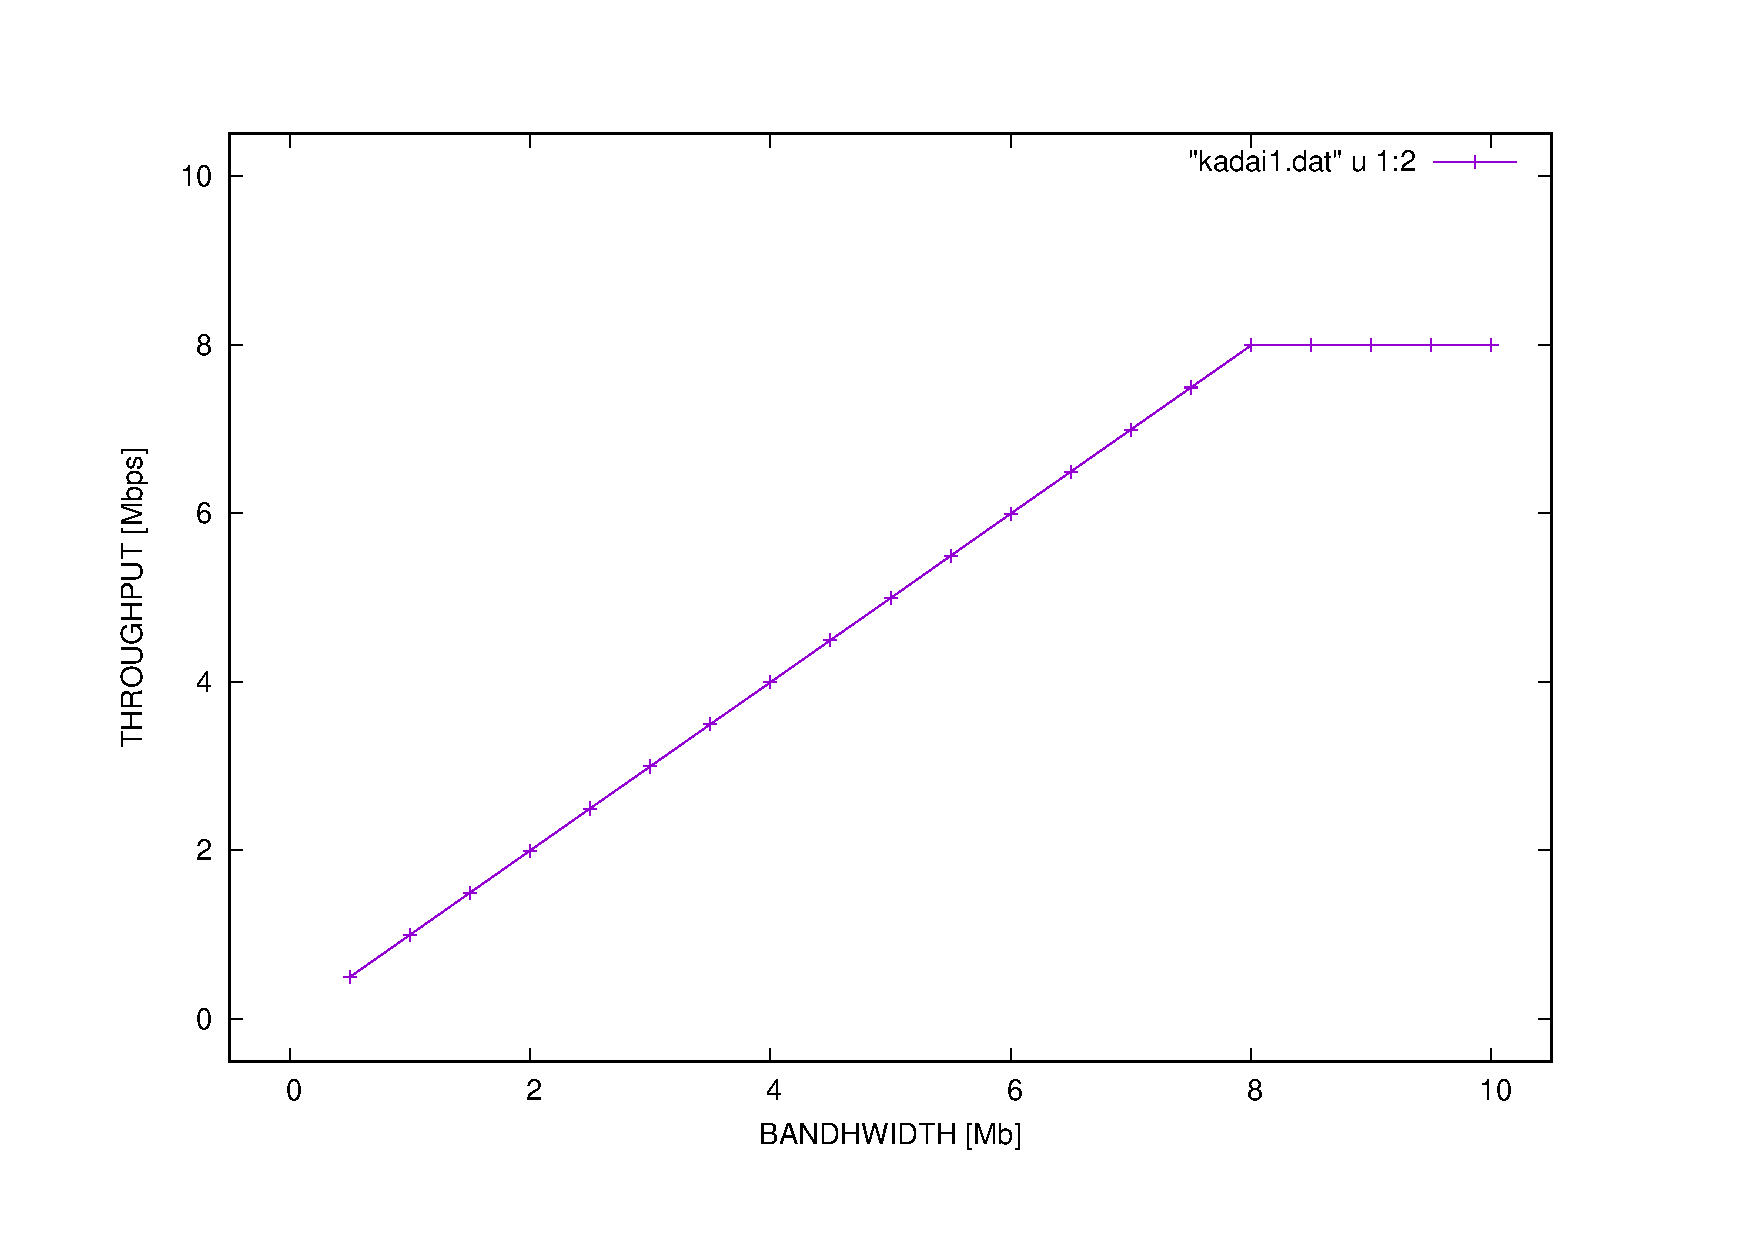
\includegraphics[width=\linewidth]{THROUGHPUT.pdf}
    \caption{スループットの測定結果}
    \label{fig:throughput}
  \end{minipage}
  % --- 図と図の間の余白 ---
  \hfill
  % --- 右側の図 ---
  \begin{minipage}[b]{0.48\linewidth}
    \centering
    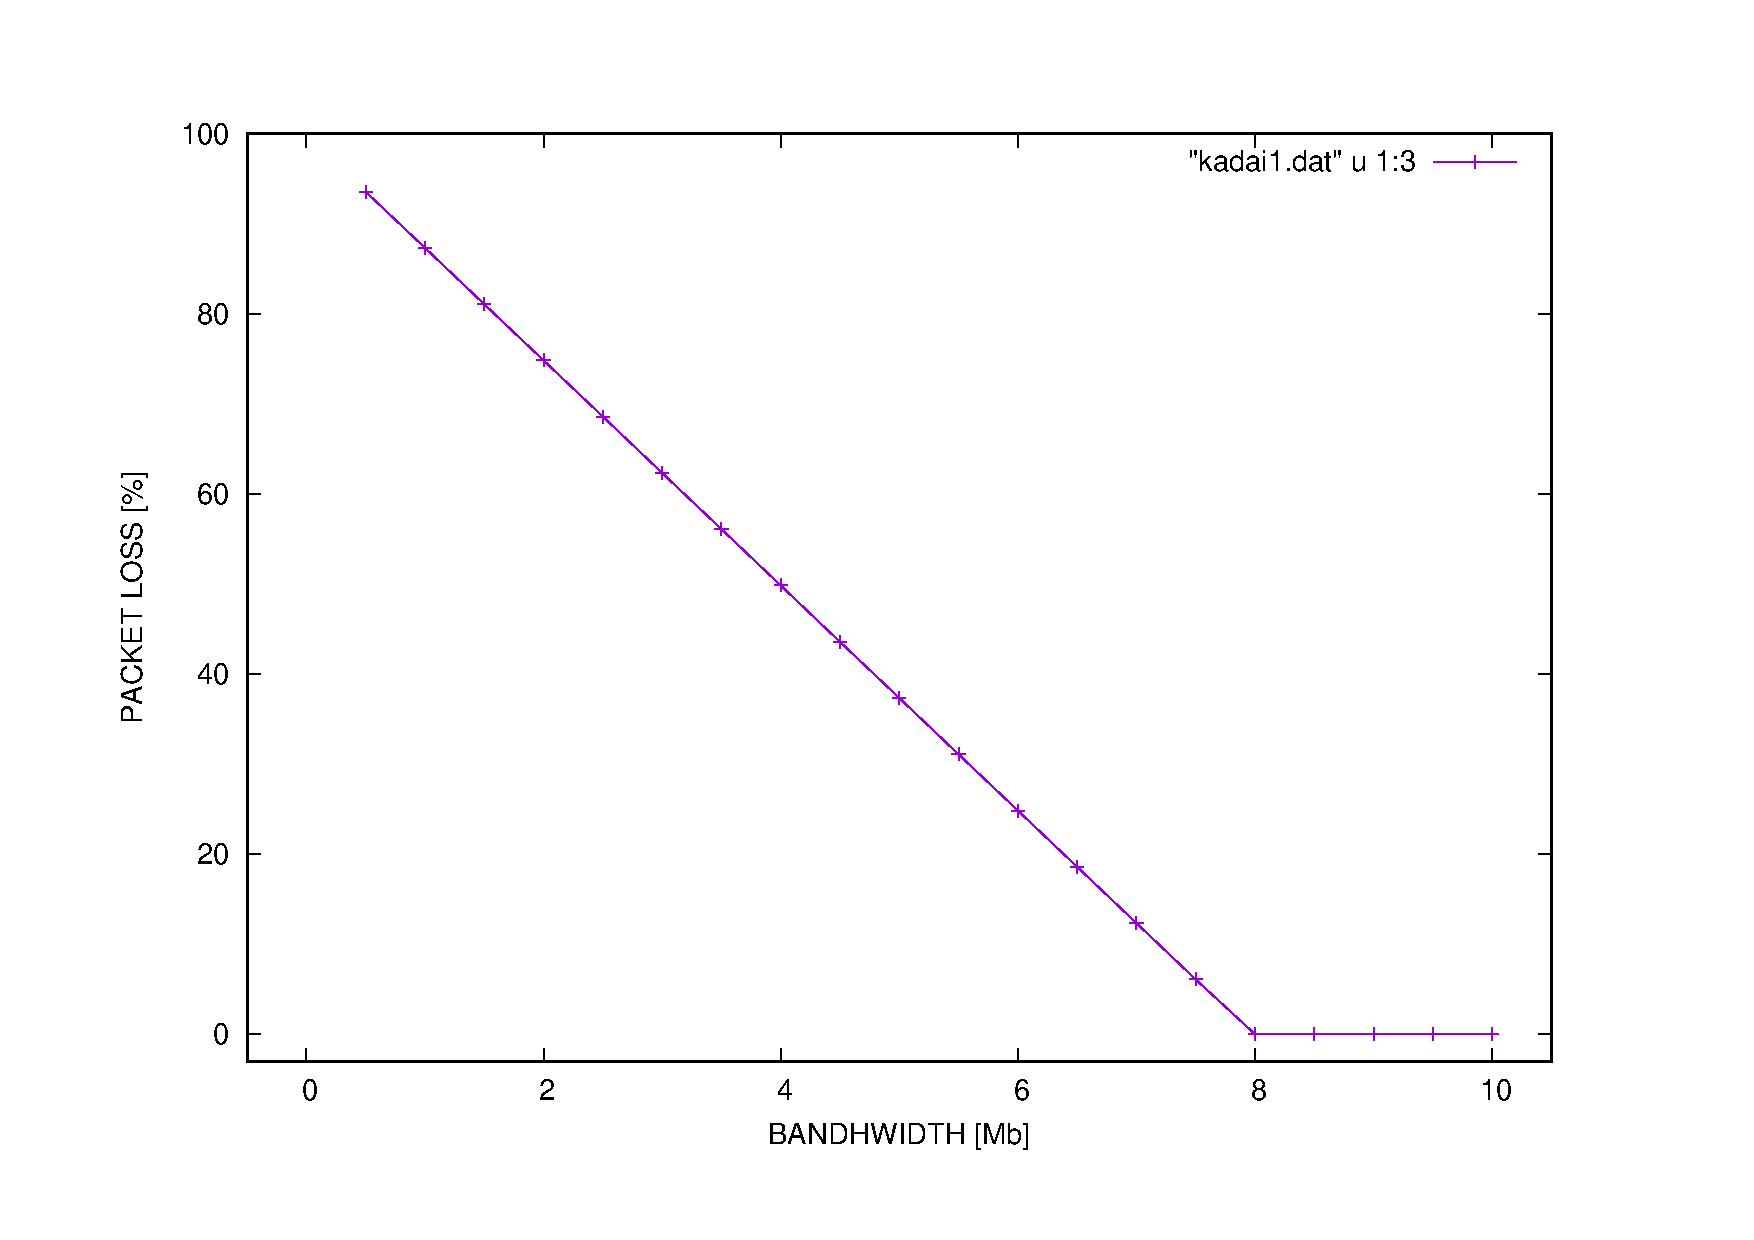
\includegraphics[width=\linewidth]{PACKET_LOSS.pdf}
    \caption{パケット損失率の測定結果}
    \label{fig:packet_loss}
  \end{minipage}
\end{figure}

\subsection{考察}
以上のデータから，以下のことがわかる．
\subsubsection{スループット}
帯域幅に比例してスループットが上昇するが，ある点からは上昇率が著しく小さくなるか$0$\texttt{Mb}になっていることがわかる．帯域幅とは$1$度に送られるデータの物理的な速さのことを指し，伝送速度とも呼ばれる$_{\text{文献}\cite{TCP_IP}}$．それが上昇することはバッファに格納される時間が短くなることを指すため，スループットが途中までは上昇している．途中からスループットが上昇していない，もしくは上昇量が小さくなる理由は，合計で送信されるデータに対して帯域幅が大きすぎるため時間あたりに送られるデータが上昇しなくなったためであると考えられる．

\subsubsection{パケット損失率}
パケット損失率についてはスループットと逆で帯域幅に対して反比例の関係になっていることがわかる．そして，パケット損失率もある時点から$0\%$になっていることがわかる．これは帯域幅が小さい場合はバッファに先に格納されているデータがフォワードされないため，あとからフォワードされたデータがバッファ内に溜まり，溢れていまいドロップするからであると考えられる．こちらもある時点から$0\%$になるがその理由としては極端に帯域幅が大きくなったことによりほとんどバッファに溜まること無くフォワードされるためであると考えられる．実際の通信では他の理由で伝送途中でデータが喪われるケースが存在するが今環境についてはそのようなケースは存在しない．

\subsubsection{総合的な考察}
スループットが上昇しなくなった帯域幅とパケット損失率が$0\%$になった帯域幅はグラフから同じと判断できる．これはこの通信におけるデータ量を上回ったからであると考えられる．

\begin{thebibliography}{99}
  \bibitem{TCP_IP} マスタリングTCP/IP 入門篇 第5版，竹下隆史・村山公保・荒井透・苅田幸雄，株式会社オーム社，平成26年5月20日
\end{thebibliography}

\end{document}
